\documentclass[10pt,oneside]{IEEEtran}
\usepackage[utf8]{inputenc}
\usepackage[T1]{fontenc}
\usepackage{listings}
\usepackage{courier}
\usepackage{color,soul}
\usepackage{algpseudocode}
\usepackage[ruled]{algorithm}
\usepackage{amssymb}
\usepackage{graphicx}
\usepackage{hyperref}
\usepackage{booktabs}
\usepackage{multirow}

%Path in Unix-like (Linux, OsX) format
\graphicspath{ {images/} }

\usepackage[
backend=biber,
style=numeric,
sorting=ynt,
citestyle=numeric
]{biblatex}
\addbibresource{ref.bib}



\lstset{basicstyle=\footnotesize\ttfamily,breaklines=true,numbersep=1em,xleftmargin=2em,xrightmargin=2em}

\title{Applying Static Analysis Techniques to Aid Clafer Modelers}
\author{Jordan A. Ross \\j25ross@uwaterloo.ca}
\date{July 28th, 2015}

\begin{document}

\maketitle
\newpage

\section{Introduction}
In this paper we provide an overview for the software reliability course project in which static analysis
is incorporated in the Clafer tool chain to aid users in modeling. Static analysis has become a popular
tool in recent years for finding bugs and discouraging bad programming practices \cite{8}.
The attractiveness of static analysis is that recent research has shown the effectiveness of tools
such as FindBugs which aim to catch simple programming errors \cite{6}. At the same time, FindBugs
and other tools such as Coverity also has sophisticated analysis to catch more serious errors in programs.

This project and paper aims to first understand the difference between tools such as FindBugs and Coverity
and in which aspects they excel. Secondly, I attempt to apply these static analysis techniques to Clafer, a
lightweight modeling language. The goal is to show that these techniques can be applied to modeling languages
to aid users that may make simple mistakes as they learn or help more experienced users from committing serious
errors.

Applying static analysis techniques is important to Clafer in order to aid users in finding possible errors in there model that the compiler does not catch. Clafer, like a traditional programming language such as C++ or Java has underlying semantics. Howerver there are cases in which semanticaly the model is correct but not what was intended by the modeler. The consquences of such errors in C++ or Java is a possible run-time exception whereas in Clafer it may lead to generation of a suboptimal or infeasible solution.

The paper is structured as follows: it begins with an overview of the Clafer lanaguage and its current use
cases. Section 3 then gives an overview and a comparision of existing static analysis techniques with a focus
on the driving forces behind Coverity and FindBugs. Section 4 proposes how theses techniques could be applied
to Clafer and the possible benifits in doing so. Section 5 then goes into the implementation details of how
we incorparted this analysis into the Clafer tool chain. Section 6 gives some results of our implemention on
various models and discussion. The paper is then concluded in Section 7.

\section{Clafer Overview}
Clafer (\underline{cla}ss, \underline{fe}ature, \underline{r}eference) is a lightweight modeling language.
The original driving force behind the development of Clafer was feature modeling and product-line modeling.
Now, Clafer is used to model a wide range of doamins as it is not a domain specific language like EAST-ADL
or AADL. The language of Clafer has minimialistic syntax and has the support of
formal semantics \cite{9}.
% Maybe explain how it builds on Alloy?

One of the key features of Clafer is the rich support for modeling variability. The following subsections
will use examples to help describe some of the Clafer constructs that are of importance in this paper.
For a more formal semantic defintion of the language and complete overview, see \cite{10}.
Throughout this paper the running example of a automotive architecture will be used.

\subsection{Concrete and Abstract}
In Clafer everything is a \textit{Clafer}\footnote{We use the italic \textit{Clafer} to denote the construct
and the plain Clafer to denote the language} and there are two types, abstract and concrete. An abstract
\textit{Clafer} can be thought of as a type (or a class in object oriented programming). A concrete
\textit{Clafer} represents a concrete element in the model. These concrete elements will result in an
instance of the model. Concrete \textit{Clafers} can be typed using abstract ones (see the next section
for more details). Listing \ref{lst:concreteAbstract} shows a concrete and abstract example in the
context of a software component.

\begin{lstlisting}[label={lst:concreteAbstract},caption={Example of abstract and concrete \textit{Clafers}}]
abstract SoftwareComponent
  xor language
    Java
    Python
    Ruby
mainComponent
\end{lstlisting}

The above listing also shows that concrete \textit{Clafers} can be nested under and abstract \textit{Clafer} (They can also be nested under concrete ones). The \lstinline$xor lanaguage$ is a group cardinality constraint that says that the language is either Java, Python, or Ruby exclusively.

\subsection{Inheritance}
Similiar to that of UML, Clafer provides first class support for inheritance. In the previous
example we had a \lstinline$mainComponent$ which should be a software component. Thus we can
\textit{type} it using inheritance. Listing \ref{lst:inheritanceEx} shows how this can be done.

\begin{lstlisting}[label={lst:inheritanceEx},caption={Inheritance example}]
abstract SoftwareComponent
  xor language
    Java
    Python
    Ruby
mainComponent : SoftwareComponent
\end{lstlisting}

When we inherit from an abstract \textit{Clafer} all children of the abstract are then apart of the concrete \textit{Clafer} as well. For example, a valid instance given the model in Listing \ref{lst:inheritanceEx} would be as follows:
\begin{verbatim}
=== Instance 1 Begin ===

mainComponent
  language
    Ruby

--- Instance 1 End ---
\end{verbatim}

\subsection{Cardinality}
Clafer also has support for expressing cardinality of \textit{Clafers} which is similiar to
that of adding multiplicies in UML. Continuing the simple example, a new type \lstinline$Function$ can be introduced
and \textit{nested} under \lstinline$mainComponent$. Furthermore, a cardinality can be given to
\lstinline$function$ to express that there are 1 or more functions in the main component.
Listing~\ref{lst:cardinalityExample} shows the example expressing this.

\begin{lstlisting}[label={lst:cardinalityExample},caption={Example of nesting and cardinality}]
abstract SoftwareComponent
abstract Function

mainComponent : SoftwareComponent
  function : Function 1..*
\end{lstlisting}

\subsection{References}
References are a key feature to Clafer as they allow modelers to express relationships between
\textit{Clafers} that may not be an ownership relationship. When you have a have nesting and a colon is used then it signfies that the parent owns the child (it instantiates the \textit{Clafer}). A reference however only means that the parent \textit{Clafer} owns a \textit{reference} to another \textit{Clafer}. References are also overloaded to allow for using integers in the language. In the previous section, cardinality and nesting were introduced but the example is maybe not the best representation of a software component. For example, a modeler may want every \lstinline$SoftwareComponent$ to be composed of 1 or more functions. Then in an instance of \lstinline$mainComponent$ the modeler might want to specify which functions are in the main component. This is done through the user of references and Listing~\ref{lst:referenceExample} shows how this would be done in Clafer. In this listing a constraint is used which is explained in more detail in the following section.

\begin{lstlisting}[label={lst:referenceExample},caption={Example use of references}]
abstract Function
abstract SoftwareComponent
  function -> Function 1..*

mainComponent : SoftwareComponent
  mainFunction : Function
  auxFunction : Function
  [function = (mainFunction, auxFunction)]
\end{lstlisting}

\subsection{Constraints}
Constraints come in different forms and are used throughout the language even though the modeler may be
unaware. For example, when a \textit{Clafer} is nested under another a constraint is imposed that every
instance of the parent \textit{Clafer} must have the child present. In the previous section, an explicit
constraint was used to assign what functions belonged to \lstinline$mainComponent$. Constraints can
take many forms and the reader should see \cite{1} for a full list of constraints
supported by the language.
\subsection{Backend Tool Support}
Clafer alone requires no tool support and much like UML can be written down on just pen and paper.
However, the tool support for Clafer allows a user to give a model written in Clafer and to generate
all valid instances of the model. Currently the Clafer tool chain supports two backends, Alloy 4.1
\cite{4} and Choco CSP \cite{3}. The Choco backend also allows for
multi-objective optimization. Figure~\ref{fig:claferToolChain} shows how the Clafer file is taken in in a \textit{.cfr} format and compiled into Alloy and Choco format (or both). Then using the dedicated instance generator the set of valid instances is generated in plain text format.
\begin{figure}[h]
  \label{fig:claferToolChain}
  \caption{Block diagram showing the Clafer tool chain work flow}
  \centering
  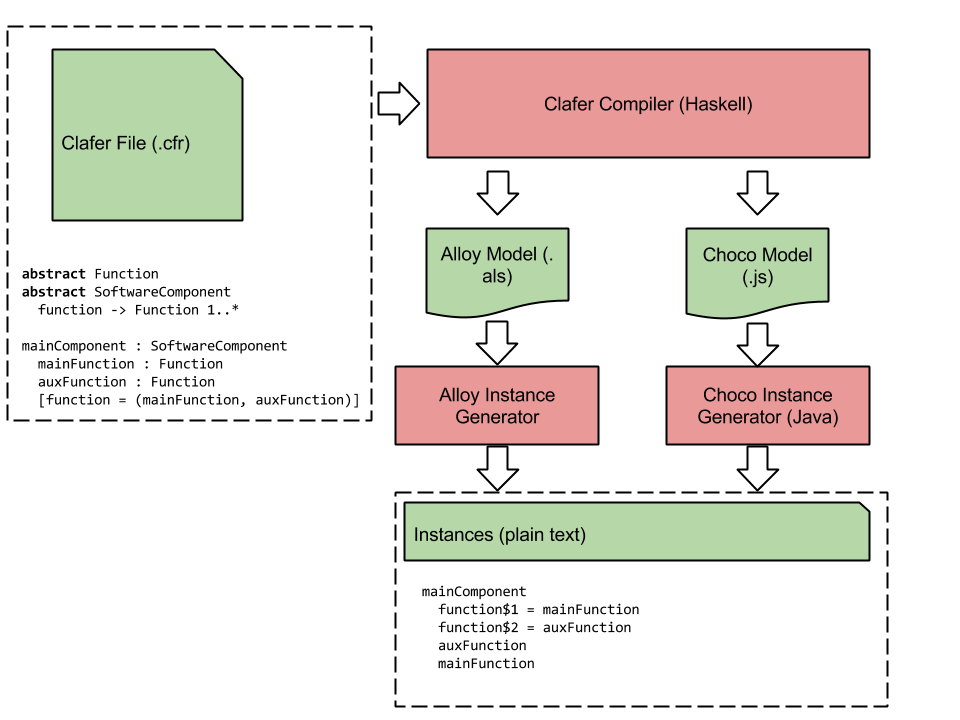
\includegraphics[width=0.5\textwidth]{ClaferToolChainWorkFlow}
\end{figure}

\section{Static Analysis Techniques}
In this section of the report an overview of some of the state of the art static analysis techniques
are examined. Static analysis has been used heavily in programming over the years, one of the most
common analysis was the analysis of types in a program and ensuring that a program can be typed checked.
A program being type checked (or saying that a program is typeable) gives a guarentee that the program
will behave properly at runtime \cite{2}.

In the past decade or so though a lot of focus and work has been done in trying to detect the presence of bugs that traditional type system may not catch \cite{8}. This work has led to at least two successful and popular tools in industry, namely FindBugs and Coverity. Both tools are static analysis tools that perform some static analysis that does not necesarily provide a guarentee that the program will behave properly at runtime, but rather probable bugs that the developer(s) may have made. The following two subsections describe two of the prevelant techniques used in both Coverity and FindBugs and why they are effective. The last subsection describes both tools in more detail and comparison between the two.

%TODO: I am thinking that we should combine the specification sections and then have a section on the static analysis techniques such as dataflow analysis and controlflow.
\subsection{Specific Specifications}
In 2000 Engler et. al. proposed a methodology and implementation for \textit{meta-level compilation} (MC) \cite{5}. MC was proposed as the authors wanted to find a way to check properties in the code such as ``interrupts must be enabled after being disabled". Of course, testing can help find some of these bugs in production code but many tests are required for all of the exection paths of the code to test this property. Also, the authors point out that one could build a rigorous specification of the program and then use model checkers to verify \cite{5}. A rigorous specification is costly and usually difficult to create so many industies don't create them.

MC is a lower cost solution that takes as input some specifications or properties written by the developer (in some pattern matching language). In the paper the authors use \textit{metal} for their implementation \cite{5}. This approach thus doesn't require the developer (or project lead) to write a formal specification for the entire program but rather just a few critical properties such as interrupts and locks.

In \cite{5} they also test their implementation on large open source projects such as Linux and OpenBSD. In doing so they found that this technique at a local level was useful in finding certain bugs with low false postive rates.

% Talk about difference between local and global analysis.

Overall MC is rather useful and succesful static analysis technique for finding real bugs in well-tested and frequently used software. It is curious though that some of the properties that the authors wanted to check had very good false positive rates while others, such as checking mutex's was very poor \cite{5}.

Another approach of having specific specifications comes from the work of Hovemeyer and Pugh. In \cite{6} they propose to investigate simple static analysis techniques for finding bugs based on the notion of \textit{bug patterns}. These patterns are concrete specifications that should hold for the code that is analyzed. In the paper the authors highlight several of the patterns the check for with their tool FindBugs. One of the concrete examples of a bug that was found in build 13 of Sun's JDK 1.6 is infinite recursion \cite{8}. Consider the following as an example:
\begin{lstlisting}[language=Java]
public String foundType() {
  return this.foundType();
}
\end{lstlisting}

% Include some more about the FindBugs detectors and some of the simpler patterns they use.

Unlike \cite{5}, in this implementation they are running conducting the analysis and pattern matches on the byte code of Java whereas Engler et. al. were writing specifications for the \textit{g++} compiler and linking to it.
\subsection{Inferring Specifications}
In 2001 Engler built on his previous work in \cite{5} to propose another static analysis technique to help find more bugs in code. Engler et. al introduced the concept of \textit{beliefs} which is the notition of inferring what the programmer intended to do in the code \cite{7}. The authors propose two types of beliefs, MAY and MUST beliefs. MUST beliefs are much like some of the bug patterns and meta-level compilation. A concrete example would be that a pointer null dereference implies that the programmer must beleive the pointer is non-null \cite{7}.

A MUST belief only requires a single contradiction (i.e. the pattern must be present only once) in order for an error to be found. This is equivelant to saying that the pattern in FindBugs must exist just one and they will throw warning or error message.
% MUST beliefs and FindBugs should be placed together I think...

MAY beliefs are the case when it is suggested that an observed pattern was programmers intent where in fact it may be a coincidence \cite{7}. A concrete example of this would be that two methods must be called together, like \textit{``a" must be followed by a call to ``b"}. In \cite{7} the approach is to treat all MAY beliefs as MUST beliefs, thus record an error everything this belief is violated, then using statistical analysis the number of false positives (coincidences) are reduced.

The analysis performed in \cite{7} is different than that of MC in the fact that a template based approach is used to mine MAY beliefs. For example, we may not know what ``a" or ``b" is in the pattern but we want to observe they are called in the same order, or if they are simply called together.

\subsection{Dataflow Analysis and Abstract Syntax Tree Traversal}
% Key points to hit:
% May beliefs.
% Dataflow analysis
% AST analysis
% The statistical analysis to reduce false positives.

\subsection{FindBugs and Coverity}
% Key points to hit:
% See if we can find projects that they were both run on and provide some graphic
% Provide a table given criteria where maybe they may differs
% Reference the Coverity slides and the paper that compares the 2 for concurrency
In this section we present some literature and studies that were found in comparing the two tools. Along with some of the data of the comparison, some thoughts are given to why the statistics could be the way they are. In a study by Al Mamun et. al. in \cite{11} they compared FindBugs, Coverity, Jlint, and Jtest. The benchmark programs that they used in their study were a set of benchmark programs introduced by Eythani et. al. The reader should refer to \cite{11} for the complete set of benchmark programs used. Table~\ref{tbl:concurrencyBugCompare} shows the results of the study with only the Coverity and FindBugs taken into consideration. Also, in the paper Al Mumun et. al. define a \textit{defect detection ratio} which is given in Equation~\ref{eq:defectDetecRatio}.
\small
\begin{equation}
  \label{eq:defectDetecRatio}
  Defect\ detection\ ratio = \frac{No.\ of\ defects\ detected\ by\ SA\ tool}{Total\ number\ of\ defects}
\end{equation}
\normalsize

\begin{table*}[ht]
\centering
\caption{Comparison of Coverity and FindBugs using the results found in \cite{11} based on a set of benchmark concurrency programs.}
\label{tbl:concurrencyBugCompare}
\begin{tabular}{@{}lllcc@{}}
\toprule
\multicolumn{1}{c}{\multirow{2}{*}{{\bf Bug Category}}}                 & \multicolumn{1}{c}{\multirow{2}{*}{{\bf Bug Type}}} & \multirow{2}{*}{{\bf Total No. Bugs}} & \multicolumn{2}{c}{{\bf No. of Bugs Detected}} \\ \cmidrule(l){4-5}
\multicolumn{1}{c}{}                                                    & \multicolumn{1}{c}{}                                &                                       & \multicolumn{1}{c|}{Coverity}    & FindBugs    \\ \midrule
\multicolumn{1}{l|}{\multirow{4}{*}{Data Race and Atomicity violation}} & \multicolumn{1}{l|}{Wrong Lock/No Lock}             & \multicolumn{1}{l|}{5}                & \multicolumn{1}{c|}{3}           & 2           \\ \cmidrule(l){2-5}
\multicolumn{1}{l|}{}                                                   & \multicolumn{1}{l|}{Double checked locking}         & \multicolumn{1}{l|}{1}                & \multicolumn{1}{c|}{0}           & 1           \\ \cmidrule(l){2-5}
\multicolumn{1}{l|}{}                                                   & \multicolumn{1}{l|}{Condition for wait}             & \multicolumn{1}{l|}{1}                & \multicolumn{1}{c|}{0}           & 1           \\ \cmidrule(l){2-5}
\multicolumn{1}{l|}{}                                                   & \multicolumn{1}{l|}{Use of deprecated methods}      & \multicolumn{1}{l|}{1}                & \multicolumn{1}{c|}{1}           & 0           \\ \midrule
\multicolumn{1}{l|}{Deadlock}                                           & \multicolumn{1}{l|}{Notify instead of notifyAll}    & \multicolumn{1}{l|}{1}                & \multicolumn{1}{c|}{0}           & 1           \\ \midrule
\multicolumn{2}{l|}{Total}                                                                                                    & \multicolumn{1}{l|}{9}                & \multicolumn{1}{c|}{4}           & 5           \\
\multicolumn{3}{l}{Overall Defect detection ratio}                                                                                                                    & 0.444                            & 0.556       \\ \bottomrule
\end{tabular}
\end{table*}

As well as the study discussed above, a comparsion from Coverity with FindBugs was also retreived in \cite{12}. In this presentation Coverity runs a comparison of Coverity with FindBugs on the Jenkins 1.496 core code on both tools with the latest version (in December 2012). Table~\ref{tbl:coverityCompare} shows the results of this comparison and it can be seen that Coverity out perfroms FindBugs in finding critical defects such as concurrency and unhandled exceptions. This corresponds to what was also seen in the study done by Al Mamun et. al. as well. However, FindBugs far surpasses Coverity in the finding of coding standard violations, best practice violations, etc. The reason for this could be that Coverity does a lot of inferring of specification as FindBugs is built on having a library of patterns that are matched against the Java byte code.

\begin{table*}[ht]
\centering
\caption{Comparison of Coverity and FindBugs on Jenkins v1.496. The data belongs to Coverity}
\label{tbl:coverityCompare}
\begin{tabular}{@{}llll@{}}
\toprule
\multirow{2}{*}{}                                                  & \multicolumn{3}{c}{{\bf Defects Found}}        \\ \cmidrule(l){2-4}
                                                                   & {\it Coverity} & {\it FindBugs} & {\it Shared} \\ \midrule
\multicolumn{1}{l|}{{\it Unhandled Exceptions (incl. NULL deref)}} & 79             & 7              & 5            \\ \midrule
\multicolumn{1}{l|}{{\it Resource Leaks}}                          & 86             & 12             & 13           \\ \midrule
\multicolumn{1}{l|}{{\it Concurrency Problems}}                    & 22             & 10             & 9            \\ \midrule
\multicolumn{1}{l|}{{\it Coding Standards, Best Practices, Other}} & 9              & 598            & 1            \\ \midrule
{\it Total}                                                        & 196            & 627            & 28           \\ \bottomrule
\end{tabular}
\end{table*}

\section{Static Analysis of Clafer}
% This section should come directly from the possible patterns markdown document.
In this section we present how static analysis could be incorporated into the Clafer tool chain and possible patterns to highlight the motivation for doing so. Since Clafer is a constraint based modeling language, there is no need for dataflow analysis. Instead, the abstract syntax tree (AST) can be traversed to look for the specified patterns. In the following four subsections each pattern is described with an example and some motivation for why the pattern is important to detect. We leave the details of how the patterns and analysis techniques are carried out to the next section.%The last subsection describes what static analyis technique will be needed in order to warn users about these pattern violations.
%TODO: Should we have a section about what static analysis techniques we are going to use?

\subsection{Pattern 1: Missing Constraint from Inherited Clafer}
The first pattern is detecting when a user may have missed a constraint when creating a concrete instance of an abstract \textit{Clafer}. The following example in Listing~\ref{lst:pattern1Ex} shows a possible scenario where this might happen.
\begin{lstlisting}[label={lst:pattern1Ex},caption={Example of Pattern 1}]
abstract Location
abstract Edge
  location -> Location 2
  length ->> int

abstract HarnessEdge : Edge
  area ->> int

Harness
  l1 : Location
  l2 : Location
  l3 : Location

  e1 : HarnessEdge
    [length = 1]
    [area = 2]
  e2 : HarnessEdge
    [location = (l2, l3)]
    [length = 1]
    [area = 3]
\end{lstlisting}
The problem with this example is the \lstinline$e1$ can take any location that is defined which is a mistake. This could be a problem if the model is very large as it will exponentially increase the search space. What is possibly worse is the fact that when doing optimization it could give a solution that is not valid for our modeled system.

In order to catch this error the AST would need to be traversed for each concrete \textit{Clafer} that inherits for an abstract one. Then for each concrete the analysis would detect any missing constraints on on which child \textit{Clafer} of the inherited \textit{Clafer}. Once all violations are found (treating these MAY beliefs as MUST beliefs), statistical analyis would be performed to reduce the number of false positives. Section~\ref{sec:implementation} discusses the details of the implementation in more detail.

\subsection{Pattern 2: Missing ``.ref" of Clafer}
The second pattern deals with references between two \textit{Clafers}. In C++, to get the value of a reference you must dereference the pointer. Much like C++, in \textit{Clafer} in order to get the \textit{Clafer} that a reference is pointing to a ``.ref" must be used. One of the limitations of the Clafer type system is that there are cases where a constraint will type check but in fact it is not constraing what the user intended. The example in Listing~\ref{lst:pattern2Ex} shows a possible scenario where this could happen.
\begin{lstlisting}[label={lst:pattern2Ex},caption={Example of Pattern 2},numbers=right]
abstract DeviceNode
abstract FunctionalAnalysisComponent
    deployedTo -> DeviceNode
abstract Command
    sender -> FunctionalAnalysisComponent
    receiver -> FunctionalAnalysisComponent
    deployedTo -> LogicalDataConnector ?
        [parent in this.deployedFrom]
    [(sender.deployedTo = receiver.deployedTo) <=> no this.deployedTo]
\end{lstlisting}

In this example the user is trying to state ``The command should not be deployed to a logical data connector if and only if the sender and receiver are not deployed to the same device node". Line 9 will type check because both sides of the equals sign are references to DeviceNode. However, the user most likely intended to compare the concrete \textit{Clafers} that \lstinline$deployedTo$ referenced. Much like pattern 1, this is a major issue because the model will compile and the user will have no idea unless they check the instances generated. This again may be easy to do for smaller models, but as they grow this becomes unrealistic.

In order to catch this error the AST would need to be traversed looking for the pattern of when equality is expressed between two reference \textit{Clafers}. This analysis would always throw the error if this pattern is seen and the user would have the option to dismiss if this was intended.
%TODO: Rewrite this maybe once we have the implementation?
\subsection{Pattern 3: Missing implies restricts variability}
One of the key features of Clafer is it's ability to easily express variability in a model. However, Clafer has it's limitations and a user should be aware when the model is not modeling the amount of variability that the user intended. The example shown in Listing~\ref{lst:pattern3Ex} highlights a possible scenario.
\begin{lstlisting}[label={lst:pattern3Ex},caption={Example of Pattern 3}]
[fa.PinchDetectionFA.PositionSensor.deployedTo.ref = ht.dn.Motor]
\end{lstlisting}

The problem with this example is that \lstinline$PinchDetectionFA$ is an optional \textit{Clafer} that is constrained by some other \textit{Clafer} in the model. Now what is trying to be modeled is that a constraint needs to be applied to the nested \lstinline$PositionSensor$ \textbf{if} the \lstinline$PinchDetectionFA$ is present in the instance. Sometimes the solver will not be smart enough to handle this case so we need to put an implies constraint to be more explicity as follows:
\begin{lstlisting}[]
[fa.PinchDetectionFA => fa.PinchDetectionFA.PositionSensor.deployedTo.ref = ht.dn.Motor]
\end{lstlisting}

The reason for this pattern is quite obvious as the user may be totally unaware of the restrictions on the variability and thus the solver is returning possibly non-optimal solutions.

In order to catch this mistake a similiar approach to the Pattern 2 will be taken and each violoation will be treated as an error and the user will be warned about the possibility of restricted variability.

\subsection{Pattern 4: Incorrect use of ``=", should use ``in"}
The last pattern that is examined is one that will help aid users who are unfamiliar with the semantics of Clafer, more specificatly with the operators ``=" and ``in". Listing~\ref{lst:pattern4Ex} highlights a scenario that a user may make.
\begin{lstlisting}[label={lst:pattern4Ex},caption={Example of Pattern 4},numbers=right]
abstract FunctionalAnalysisComponent
  deployedTo -> DeviceNode
    [parent in this.deployedFrom]

abstract DeviceNode
  deployedFrom -> FunctionalAnalysisComponent *
    [this.deployedTo = parent]

function1 : FunctionalAnalysisComponent
  [deployedTo = (device1, device2)]

device1 : DeviceNode
device2 : DeviceNode
\end{lstlisting}

The example is incorrect because line 10 should be \lstinline$[deployedTo in (device1, device2)]$. The reason it should be this is that deployedTo should only be in the set of device1 and device2. What is currently written in the model is that deployedTo should contain both elements of the set device1 and device2 which is unsatisfiable. Therefore the solver will return 0 solutions and the user will have to manually track down the error.

Much like the previous two, this pattern would use the AST to find the corresponding pattern and always throw a warning when it finds a match.

\section{Implementation}
\label{sec:implementation}
In this section the implementation of the patterns described in the previous section is described. For each pattern the algorithm is given for how the pattern was analyzed. Along with the algorithm, each pattern describes how warnings are issued to the user (i.e. if any statistical analysis or filtering is applied to the raw errors). Before the patterns are described in detail, some background information is given on where this implementation fits into the existing Clafer tool chain backends.

\subsection{Overiew and Design}
The Choco backend is Clafer's most developed backend and allows for the most functionality by having multi-objective optimization. Therefore for the scope of the course project it was chosen to plug the analysis into the Choco backend. This was also driven by the fact of the authors lack of experience in writing Haskell opposed to Java.

As seen earlier in Figure~\ref{fig:claferToolChain} the original Clafer file (in .cfr format) is Compiled and an intermediate representation of the model is outputed to a Javascript file. The Choco backend then takes the Javascript model and builds an AST and uses the AST representation to perform the solving. Since there was exisiting Java code to build the AST from the Javascript file and perfrom traversals, this implementation makes heavy use of the exisiting code base found in the \href{https://github.com/gsdlab/chocosolver/}{Choco Github repository}.

For the initial implementation of the tool it was decided to not optimize for scalability as most models were fairly small (< 200 Clafers) as opposoed to millions of lines of code that Coverity and FindBugs need to analyze. Thus each pattern carried out its analysis seperately. In future work the code will be optimized so that the number of AST traversals can be reduced.

Lastly, for patterns 2 through 4 the main AST traversal was to retrieve the set of all constraints in the model. Once the constraints were collected they were analyzed using a visitor design pattern in order to parse the many different types of expressions that a constraint can contain. For pattern 1, the traversal of the AST was more complex and is captured in the psuedocode given in the following subsection.
%TODO: Should we include a partial class diagram?

\subsection{Pattern 1 Implementation}
Recall that pattern 1 was to find instances in the model where a modeler may have mistakenly forgetten to constrain a \textit{Clafer} from its super \textit{Clafer}. The algorithm for this pattern is given in Algorithm~\ref{alg:pattern1}.

\begin{algorithm}[H]
\caption{Unconstrained Sub Clafers}\label{alg:pattern1}
\begin{algorithmic}[1]
\Procedure{analyzeUnconstrainedRefClafers}{}
  \State \textbf{let} $X$ be an order set of abstract Clafers, sub before super Clafers
  \ForAll{$X_i \in Reverse(X)$}\Comment{Loop through $X$ in reverse order}
    \If{$X_i$ has a super Clafer $X_j$}
      \State $X_i.set \gets$ \Call{findUnconstrainedRefClafersOfAbstract}{$X_i$, $X_j.set$}
    \Else
      \State $X_i.set \gets$ \Call{findUnconstrainedRefClafersOfAbstract}{$X_i$, $\emptyset$}
    \EndIf
  \EndFor
  \ForAll{$X_i \in X$}
    \State \textbf{let} $Z$ be the set of concrete Clafers that inherit from $X_i$
    \ForAll{$s \in X_i.set$}
      \ForAll{$Z_i \in Z$}
        \If{$\exists constraint(s) \in Z_i$}
          \State Log success
        \Else
          \State Log error
        \EndIf
      \EndFor
      \State Analyze warnings for $X_i$
    \EndFor
  \EndFor
\EndProcedure
\Procedure{findUnconstrainedRefClafersOfAbstract}{$a,S$}\Comment{The unconstrained Clafers of a given a propogated set of unconstrained Clafers S}
   \ForAll{$s \in S$}
    \If{$\exists constraint(s) \in a$}
      \State $S \gets S \setminus \{s\}$
    \EndIf
   \EndFor
   \ForAll{$child \in childrenWithRef(a)$}
    \If{$\nexists constraint(child) \in a$}
      \State $S \gets S \cup \{child\}$
    \EndIf
   \EndFor
   \State \Return $S$
\EndProcedure
\end{algorithmic}
\end{algorithm}

The algorithm will analyze each of the abstract \textit{Clafers} first so that that if another abstract Clafer inherits from another and constrains its super \textit{Clafers} a false positive is not thrown. The algorithm does not show how any statistical analysis that is done on the warnings log for each abstract \textit{Clafer}. In order to reduce false positives some analysis needs to be done on the logged warning messages. Algorithm~\ref{alg:pattern1Stats} describes the process of how an warning is generated based on some simple analysis.

\begin{algorithm}[H]
\caption{Analysis Procedure on Warnings for Unconstrained Reference Clafers}\label{alg:pattern1Stats}
\begin{algorithmic}[1]
\Procedure{warningAnalysis}{X}
  \State \textbf{let} $a$ be the context abstract Clafer
  \State \textbf{let} $V$ be the set of concrete Clafers that have an error logged.
  \State $successCnt \gets $ total successes for $a$
  \State $errorCnt \gets $ total errors for $a$
  \If{$successCnt != 0$}
    \State Generate warnings $\forall v \in V$
  \EndIf
\EndProcedure
\end{algorithmic}
\end{algorithm}

In the analysis we don't thow any warnings if there are no successes since its obvious the user didn't want to constrain the Clafer. More sophisticated statistical analysis is not used since the model would like to know if there are any unconstrained reference Clafers. It should be up to the modeler to determine if it was they inteded or not. In future interations of this tool it would be good if the modeler could mark warnings as intended so they are not shown up on future executions of the tool. This reasoning is valid in the context of modeling as models are not nearly as large as the industrial size code bases so a modeler could more easily traverse through the warnings to determine what was intended or not.

\subsection{Pattern 2 Implementation}
In pattern 2 the goal is to notify the modeler when they may be missing the ``.ref" on  \textit{Clafers} inside of the a constraint. Unlike in pattern 1 there is no need to do a complext AST traversal over the abtract and concrete \textit{Clafers}. Instead what is needed is the entire set of constraints that involve a ``set test". A set test is when equality (=) is assereted between two sets of Clafers. In this case, the sets are single valued sets. Algorithm~\ref{alg:pattern2} descirbes the high level approach to detecting this pattern. However, as meantion earlier, the implementation was carried out by creating a concrete vistor to an existing abstract visitor. In our concrete visitor the expression is parsed until a matching set test expression is found and analyzed.

\begin{algorithm}[H]
\caption{Finding missing ``.ref" of Clafer in Constraints}\label{alg:pattern2}
\begin{algorithmic}[1]
\Procedure{findingMissingRefOfClafers}{}
  \State \textbf{let} $C$ be the set of constraints with equality
  \ForAll{$c \in C$}
    \State $left \gets c.getLeftOfEqual()$
    \State $right \gets c.getRightOfEqual()$
    \If{$left.hasRef() \&\& right.hasRef()$}
      \If{$left || right$ does not a trailing $.ref$}
        \State log error
      \EndIf
    \EndIf
  \EndFor
\EndProcedure
\end{algorithmic}
\end{algorithm}

\subsection{Pattern 3 Implementation}
Pattern 3 was implemented in a very similiar way to pattern 2 in terms of using the visitor design pattern. For this pattern its helpful to see how the constraint is desugared for the compiler. Consider the following constraint from earlier:
\begin{lstlisting}[]
[fa.PinchDetectionFA => fa.PinchDetectionFA.PositionSensor.deployedTo.ref = ht.dn.Motor]
\end{lstlisting}
The constraint would be desugraded as follows:
\begin{lstlisting}[]
[(#fa.PinchDetectionFA >= 1) => (fa.PinchDetectionFA.PositionSensor.deployedTo.ref = ht.dn.Motor)]
\end{lstlisting}
The ``\#" sign means ``count the number of X". Thus in this constraint we want to make sure we have at least 1 \textit{PinchDetectionFA} in order to have the set test expression on the right of the implies. The above constraint is a correct constraint in terms of pattern 3, thus what is needed to throw an error is to have set test expression where either the left side of the equals is possibly optional. If a Clafer is optional it means that it must have a lower bound cardinality of 0. Furthermore there needs to not exist an implies to the left of the set test expression in which the optional Clafer is present. The part that makes this analysis tricky is that all parents of the Clafer involved in the left side of the set test expression need to be analyzed (i.e. PinchDetectionFA is the parent of PositionSensor).
%TODO: Not sure if I should have psuedocode here

\subsection{Pattern 4 Implementation}
Pattern 4 was implemented similiar to that of pattern 2. Like the last two patterns, the AST was traversed in order to retrieve the set of all constraints. Then like pattern 2, the visitor pattern was used to find a set test expression in which the right side was checked to see if it was a union expression like:
\begin{lstlisting}[]
[myComponents = (comp1 ++ comp2 ++ comp3)]
\end{lstlisting}
Then if the left side had a lower bound cardinality of 0 then a warning was generated because the empty set case was not taken into account. Algorithm~\ref{alg:pattern4} describes the high level approach for detecting the possible violations.
%TODO: Provide pseudo code.
\begin{algorithm}[H]
\caption{Finding missing ``.ref" of Clafer in Constraints}\label{alg:pattern4}
\begin{algorithmic}[1]
\Procedure{findingMissingRefOfClafers}{}
  \State \textbf{let} $C$ be the set of constraints with equality
  \ForAll{$c \in C$}
    \State $left \gets c.getLeftOfEqual()$
    \State $right \gets c.getRightOfEqual()$
    \If{$left.lowCard() == 0$}
      \If{$right.isUnionExpr()$}
        \State log error
      \EndIf
    \EndIf
  \EndFor
\EndProcedure
\end{algorithmic}
\end{algorithm}

\section{Results \& Discussion}
\begin{table*}[ht]
\centering
\caption{Evaluation of Number of Warnings Generated for 11 Realistic Clafer Models.}
\label{tbl:warningGeneratedAndSize}
\begin{tabular}{@{}l|cccccc@{}}
\multicolumn{1}{c|}{\multirow{2}{*}{{\bf Model}}} & \multicolumn{2}{c}{{\bf Size}}   & \multicolumn{4}{c}{{\bf \# Warning's Generated}}                      \\ \cmidrule(l){2-7}
\multicolumn{1}{c|}{}                             & {\it Clafers} & {\it Constraints} & {\it Pattern 1} & {\it Pattern 2} & {\it Pattern 3} & {\it Pattern 4} \\ \midrule
{\it Power Window Thesis}                         & 107           & 154               & 0               & 0               & 0               & 0               \\ \midrule
{\it Software Architecture - 1st draft}           & 33            & 25                & 0               & 2               & 0               & 0               \\ \midrule
{\it Software Architecture - 2nd draft}           & 33            & 37                & 0               & 0               & 0               & 0               \\ \midrule
{\it Data Center Resource Allocation - ISAP}      & 31            & 22                & 3               & 0               & 0               & 0               \\ \midrule
{\it Data Center Resource Allocation - SSAP}      & 21            & 13                & 3               & 0               & 0               & 0               \\ \midrule
{\it Data Center Resource Allocation - TSAP}      & 27            & 27                & 1               & 0               & 0               & 0               \\ \midrule
{\it Data Center Resource Allocation - WSAP}      & 21            & 13                & 3               & 0               & 0               & 0               \\ \midrule
{\it Power Window}                                & 136           & 152               & 4               & 0               & 0               & 0               \\ \midrule
{\it Power Window Old}                            & 117           & 88                & 0               & 2               & 0               & 0               \\ \midrule
{\it Wire Routing}                                & 83            & 77                & 4               & 0               & 0               & 0               \\ \midrule
{\it Zeller Paper Model}                          & 106           & 186               & 1               & 0               & 0               & 0
\end{tabular}
\end{table*}

The tool was first tested on a various number of test Clafer models written for the specific purpose of triggering each of the patterns and generated the correct errors. Once the test cases passed the tool was then evaluated on 11 realistic Clafer models developed by the author of this paper and previous grad student whom worked heavily on Clafer. The 11 models range in size and complexity as some were used in early courses while others are used in ongoing research and previous thesis work.

This sample should not be taken to be a representative sample of Clafer users as the two modelers, while some models are taken from early, are still considered advanced users of Clafer. As the language develops it is the hope that this tool could be evaluated on new and more experienced users of Clafer in a larger setting.

Even though the sample size was small and un-representative there were a few models that were provided some interesting results. First, the evaluation was carried out by first running the model given the tool and logging the number of errors generated by each of the patterns, as well as their model size. The results are shown in Table~\ref{tbl:warningGeneratedAndSize}.

From the table it can be seen that no warnings were generated for patterns 3 and 4. A reason that this could be is that these are two patterns that can lead to a model generating zero instances. Thus, for most of these models (since they were somewhat final versions) they may have encountered this pattern but it was not present in the final version. This is where evaluating on a new user as they develop a model from scratch could be interesting as patterns 3 and 4 could aid in debugging the model.

One interesting case that the evaluation did catch was the repair of a pattern 2 type warning from an earlier version of the \textit{Software Architecture} model to a later one. This provided some evidence that these patterns are detected manually by modelers and fixed as the model is developed.

For the next step of the evaluation each of the warnings was investigated by the author to determine if it was a false positive or not. If it was a false positive it was further classified into whether it was a \textit{true} false positive or if it was an incorrect implementation of the tool algorithm. Table~\ref{lst:falsePositive} shows the results of this evaluation (Patterns 3 and 4 were not considered since no warnings were generated).

\begin{table*}[h]
\centering
\caption{Evaluation of False Positives for Warnings Generated for Patterns 1 and 2 on 11 Realisitc Clafer Models.}
\label{lst:falsePositive}
\begin{tabular}{@{}l|llllll@{}}
\multicolumn{1}{c|}{\multirow{2}{*}{{\bf Model}}} & \multicolumn{2}{c|}{{\bf \# Warning's Generated}}                         & \multicolumn{2}{c}{{\bf \# False Positives}}                              & \multicolumn{2}{c}{{\bf Classification of False Positives}}                                        \\ \cmidrule(l){2-7}
\multicolumn{1}{c|}{}                             & \multicolumn{1}{c}{{\it Pattern 1}} & \multicolumn{1}{c}{{\it Pattern 2}} & \multicolumn{1}{c}{{\it Pattern 1}} & \multicolumn{1}{c}{{\it Pattern 2}} & \multicolumn{1}{c}{{\it Incorrect Implementation}} & \multicolumn{1}{c}{{\it True false positive}} \\ \midrule
{\it Power Window Thesis}                         & 0                                   & 0                                   & 0                                   & 0                                   & 0                                                  & 0                                             \\ \midrule
{\it Software Architecture - 1st draft}           & 0                                   & 2                                   & 0                                   & 0                                   & 0                                                  & 0                                             \\ \midrule
{\it Software Architecture - 2nd draft}           & 0                                   & 0                                   & 0                                   & 0                                   & 0                                                  & 0                                             \\ \midrule
{\it Data Center Resource Allocation - ISAP}      & 3                                   & 0                                   & 1                                   & 0                                   & 0                                                  & 0                                             \\ \midrule
{\it Data Center Resource Allocation - SSAP}      & 3                                   & 0                                   & 1                                   & 0                                   & 0                                                  & 0                                             \\ \midrule
{\it Data Center Resource Allocation - TSAP}      & 1                                   & 0                                   & 1                                   & 0                                   & 0                                                  & 0                                             \\ \midrule
{\it Data Center Resource Allocation - WSAP}      & 3                                   & 0                                   & 1                                   & 0                                   & 0                                                  & 0                                             \\ \midrule
{\it Power Window}                                & 4                                   & 0                                   & 0                                   & 0                                   & 0                                                  & 0                                             \\ \midrule
{\it Power Window Old}                            & 0                                   & 2                                   & 0                                   & 0                                   & 0                                                  & 0                                             \\ \midrule
{\it Wire Routing}                                & 4                                   & 0                                   & 3                                   & 0                                   & 3                                                  & 1                                             \\ \midrule
{\it Zeller Paper Model}                          & 1                                   & 0                                   & 0                                   & 0                                   & 0                                                  & 0
\end{tabular}
\end{table*}

As can be seen in the table there were 3 false positives that were classified as a incorrectness in the implementation of the pattern 1. The reason is that the constraint was nested in an unexpected Clafer. The algorithm thus would need to be adjusted to account for this case in future work.


\printbibliography

\end{document}
